\documentclass[a4paper]{report}

%% Language and font encodings
\usepackage[english]{babel}
\usepackage[utf8x]{inputenc}
\usepackage[T1]{fontenc}
\usepackage{graphicx}
\usepackage[english]{babel}
\usepackage[utf8x]{inputenc}
\usepackage[T1]{fontenc}
\usepackage{sectsty}
\usepackage{pdfpages}
\usepackage[section]{placeins}
\usepackage{float}% If comment this, figure moves to Page 2
\usepackage{listings}
\usepackage{caption}
\usepackage{subcaption}

%% Sets page size and margins
\usepackage[a4paper,top=3cm,bottom=2cm,left=3cm,right=3cm,marginparwidth=1.75cm]{geometry}

%% Useful packages
\usepackage{amsmath}
\usepackage{graphicx}
\usepackage[colorinlistoftodos]{todonotes}
\usepackage[colorlinks=true, allcolors=blue]{hyperref}

\title{Your Paper}
\author{You}

\begin{document}
\maketitle
\tableofcontents

\chapter{Quality Attriburtes}
\section{Some Background}
\subsection{Stakeholders}
Stakeholders represent different(typically conflicting) perspectives on the system and attemp to influence the architect. The architiect needs to tradeoff the different influences and resolve the conflict. e.g. -  Marketing might want to have a big market but maintence would prefer system to be simple. 

\begin{figure}[h]
\centering 
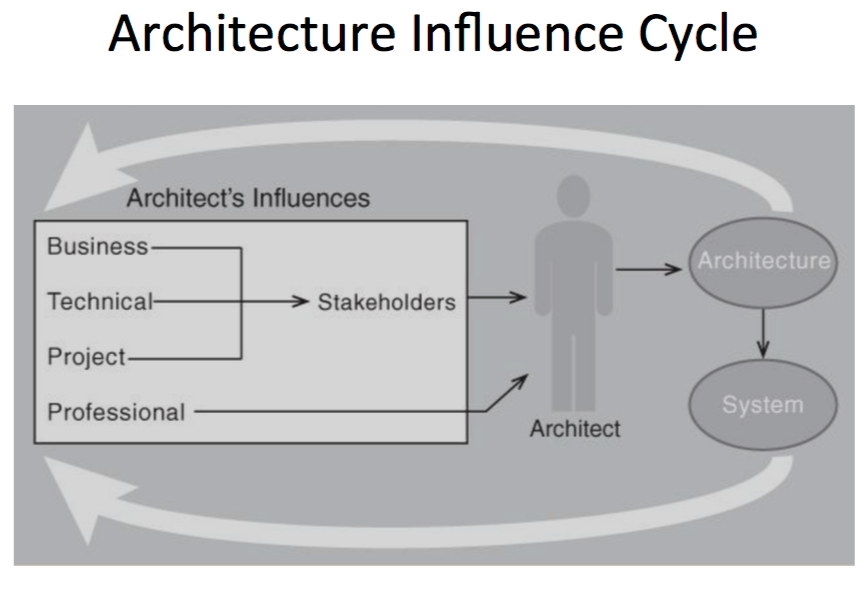
\includegraphics[scale=0.3]{aimages/influencecycle.png}
\caption{\label{tab:widgets}Architect Influence Cycle }
\end{figure}

\subsection{Functional Requirements}
these specify what the system does, architecture is important to them as they structure the containers that hold functionality !!shit in lec! !. Functional requirements are things the system does.

\subsection{Constraints}
hese are decisions that have already been taken e.g. we will use the Java programming language (because we have a Java development team available) or the system will only support certain web browsers
\section{Quality Attributes}
Quality Attributes specify, usually quantitatively, the requirements on particular bits of functionality or on the whole system. 
Software Quality Attributes are the benchmarks that describe system’s intended behavior within the environment for which it was built. The quality attributes provide the means for measuring the fitness and suitability of a product.
!!Is there a difference between QA's and Non-Fucntional requirements? !!

\subsection{Problems with Quality Attributes}
\begin{itemize}
\item Often QA's are not testable. e.g. what does it man to say something is modifiable or usable or dependable or resilient?
\item It can be difficult to map from a concern about the system to a QA. For example, a high failure rate in some transaction could be a performance issue or it could be an availability issue
\item Communities around a particular quality attribute have developed their own terminology (e.g. security has attacks, performance has events!!what?!!, etc).
\end{itemize}

\textbf{One Solution: } use quality attribute scenarios to provide sufficient specificity to avoid some of these issues.

\subsection{QA Scenarios}
QA scinario has following components:
\begin{enumerate}
\item Source of Stimulus: Person or another System
\item Stimulus: An action system responds to e.g. using the wrong configuration specification for the system.
\item Environment: Captures wider aspects of the system
\item Artifact: Part of the system that is stimulated
\item Response: Activity resulting from stimulus
\item Response measure: Measure of the response so that the scenario is testable e.g time taken to detect wrong config.
\end{enumerate}

\begin{figure}[h]
\centering 
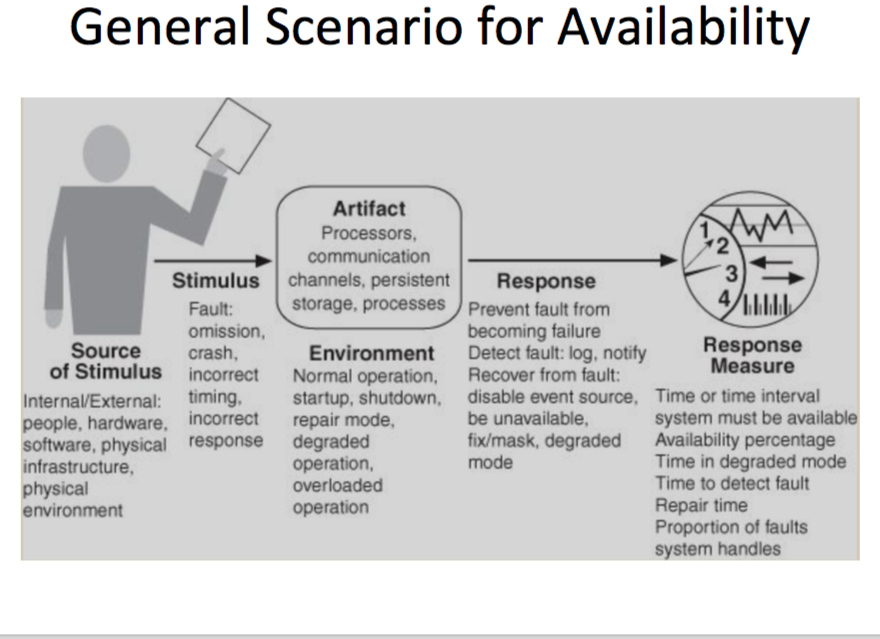
\includegraphics[scale=0.3]{aimages/qascenario.png}
\caption{\label{tab:widgets}Example QA Scenario Components}
\end{figure}


Each QA has a general scenario that it tries to capture with its components. This acts like a guide for the architect.

\subsection{Architectural Tactics} 
\begin{enumerate}
\item Artitectural tacticas are a way of documenting routes to achieve a QA requirement.
\item Architectural Tactic is a design Decision that influences the achievement of a QA response. They are more primitive than design patterns.
\item Tactics are based on single QA's and dont take trandeoffs into account.
\item Teactics are usually more generic and need to be specialised to a specific context.
\item They allow the architect to systematically enumerate possible design decision.
\end{enumerate}

\subsubsection{Example Tactics}

\subsubsection*{Example of Availaibilty Tactics}
DIfferent tactics identify different forts of reposnsibilities and how to achieve them. For exam for availaibility: 
\begin{figure}[h]
\centering 
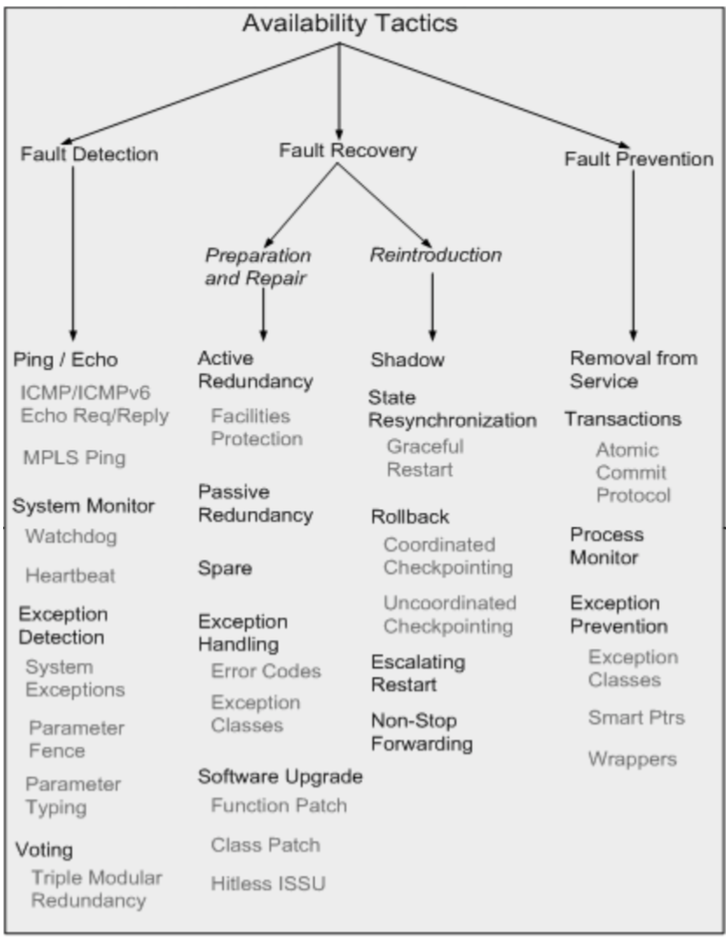
\includegraphics[scale=0.3]{aimages/availaibilitytactic.png}
\caption{\label{tab:widgets}Availaibilty Tactics}
\end{figure}

\begin{itemize}
\item Example- Watchdog times ensure the availability of systems by initialing a restart in the event of apparent inactivity.
\item Another example- Heartbeat is used in high availibility clusters to provide availaibility of a shared resource. One system owns the resource and regularly sends out heartbeat to indicate system is alive. If heartbeat is missed the backup system takes over responsibility of the shared resource.
\end{itemize}

\subsection{Categories of Architectural Design Decisions}
There are seven broad categories of design decisions:
\begin{enumerate}
\item \textbf{Allocation of responsilbilties}- identify the most important responsibilities and determine how to allocate these to runtime and static elements.
These are often specific to a QA and so the specifics depend on the QA, for example in the case of availability fault detection is an important responsibility that will be further decomposed and distributed in the architecture.
\item \textbf{Coordination Model} - Components in the architecture interact with one another via a collectioon of mechanisms. This is called the coordination model. Things it takes into account are:
\begin{itemize}
\item What elemsts in the system need to coordinate with one another.
\item What properties(eg timing, security) does the coordination need to have
\item The mechanisms and their properties(eg statefullness, synchrony, dilevery guaranties).
\end{itemize}
\item \textbf{Data Model} - How data is created, destroyed. Data acess methods, operations on the data, the properties of the data are all included in the Data Model. We also need to decide on how the data would be organised, stored, backed up and recovered in case of data loss. It also includes Maintaining Metadata that controls the interpretation of the data.

\item \textbf{Management of resources} We can have both Hardware(eg CPU, memory, battery) and Software(Buffers, Processes) resources which need to be Managed. Management includes:
\begin{itemize}
\item Identifying which resources need to be managed.
\item What system element should manage a resource.
\item Work out sharing strategies and how to arbitrate in contention situations
\item Consider the consequences of running out of a resource (e.g. Memory).
\end{itemize}

\item \textbf{Mapping Among Architectural Elements}
We have 2 types of mapping:
\begin{itemize}
\item Mapping b/w different types of elements in the architecture e.g. b/w static development structures and threads or processes
\item Mapping b/w software elements and environment elements e.g. from process to specific processors.
\end{itemize}
Some important Mappings: code to runtime structures, runtime elements to environment, data model elements to data stores.

\item \textbf{Binding Time Decisions}
!!LOOK UP AGAIN- SHIT IN LECTURES!!

\item \textbf{Choice of technology}- Important so that we can realise other decisions in a concrete system. Things to consider:
\begin{itemize}
\item What technologies are avalaible?
\item what tools are availaible to support the technologies?
\item How much training would be needed for each technology?
\item What are the consequesces and restrictions of the the choice of a technology(eg. incompatible with other tech)?
\item How does the tech fit in other technologies used in the organisation?
\end{itemize}
\end{enumerate}


\chapter{Security}
We need to consider atacks on Confidentiality,Integrity and Availability.AIacks need to be monitored andd etected, resisted where possible, otherwise we may need some other form of reaction, eventually we should be able to fully recover.
\section{Important QA's}
\begin{enumerate}
\item \textbf{Confidentiality} - Only those who should have accessare given access
\item \textbf{Integrity} -  Data or services are not subject to unauthorised manipulation.
\item \textbf{Availibility} -  The system is availble for legitimate use.
\item \textbf{Security Mechanisms} Authentication, Authorisation, non-repudation
\end{enumerate}

\section{Security Scenario Components}
\subsection{Generic Example}
\begin{figure}[h]
\centering 
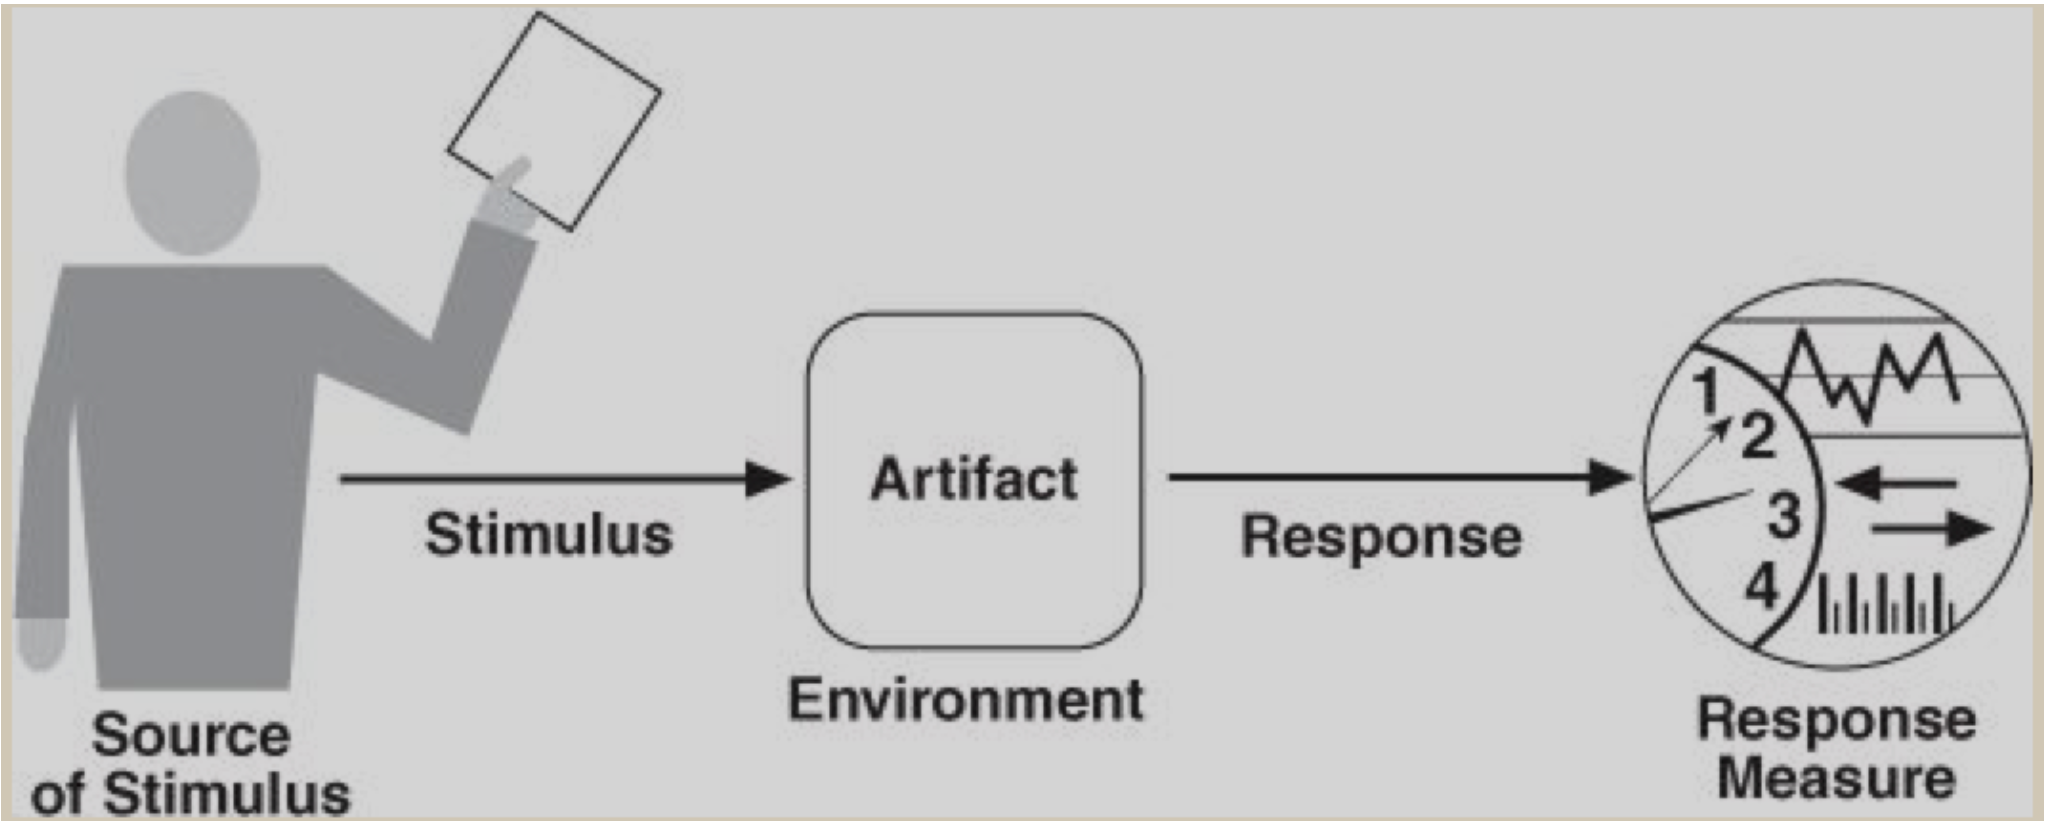
\includegraphics[scale=0.3]{aimages/genreralqascenario.png}
\caption{\label{tab:widgets} QA Scenario Components}
\end{figure}

\begin{itemize}
\item \textbf{Source}- Humans or systems that may or may not have been identified and can be either inside or outside the organisation
\item \textbf{Stimulus}- Unauthorized attempt to access, Manipulate or disable the artifact.
\item \textbf{Artifact}- System services, data, components, data produced or consumed by the system.
\item \textbf{Environment}- online, offline, connected to network, disconnected to network, behind firewall, fully/partially operating, not operational
\item \textbf{Response}- Transaction carried out s.t: Data or services protected from unauthorised access, no data manipulation without authorization, parties in a transaction are identified with assurance, Par'es cannot repudiate their participation, Data, resources etc are available for legititimate use, Appropriate people are notified when threat is identified.
\item \textbf{Response Measure}- assessment of the degree of compromise, temporal and spatial data on the compromise, how many atacks were resisted, how much data is vulnerable
\end{itemize}

\section{More Concrete example}
Assume a more concrete example fo Denial of Service. The components could be:
\begin{itemize}
\item \textbf{Source}- A wide ranfe of systems with different IP.
\item \textbf{Stimulus}- Access to the service provided
\item \textbf{Artifact}- The service we are concerened with
\item \textbf{Environment}- Normal operation
\item \textbf{Response}- Detect Normal Load
\item \textbf{Response Measure}- Mode of operation is changed to ensure normal service to trusted IP addresses.!!what?!!
\end{itemize}

\section{Security Architecture tactics}
Tactics are a high-level way of categorizing possible protection against aIack.
\begin{figure}[h]
\centering 
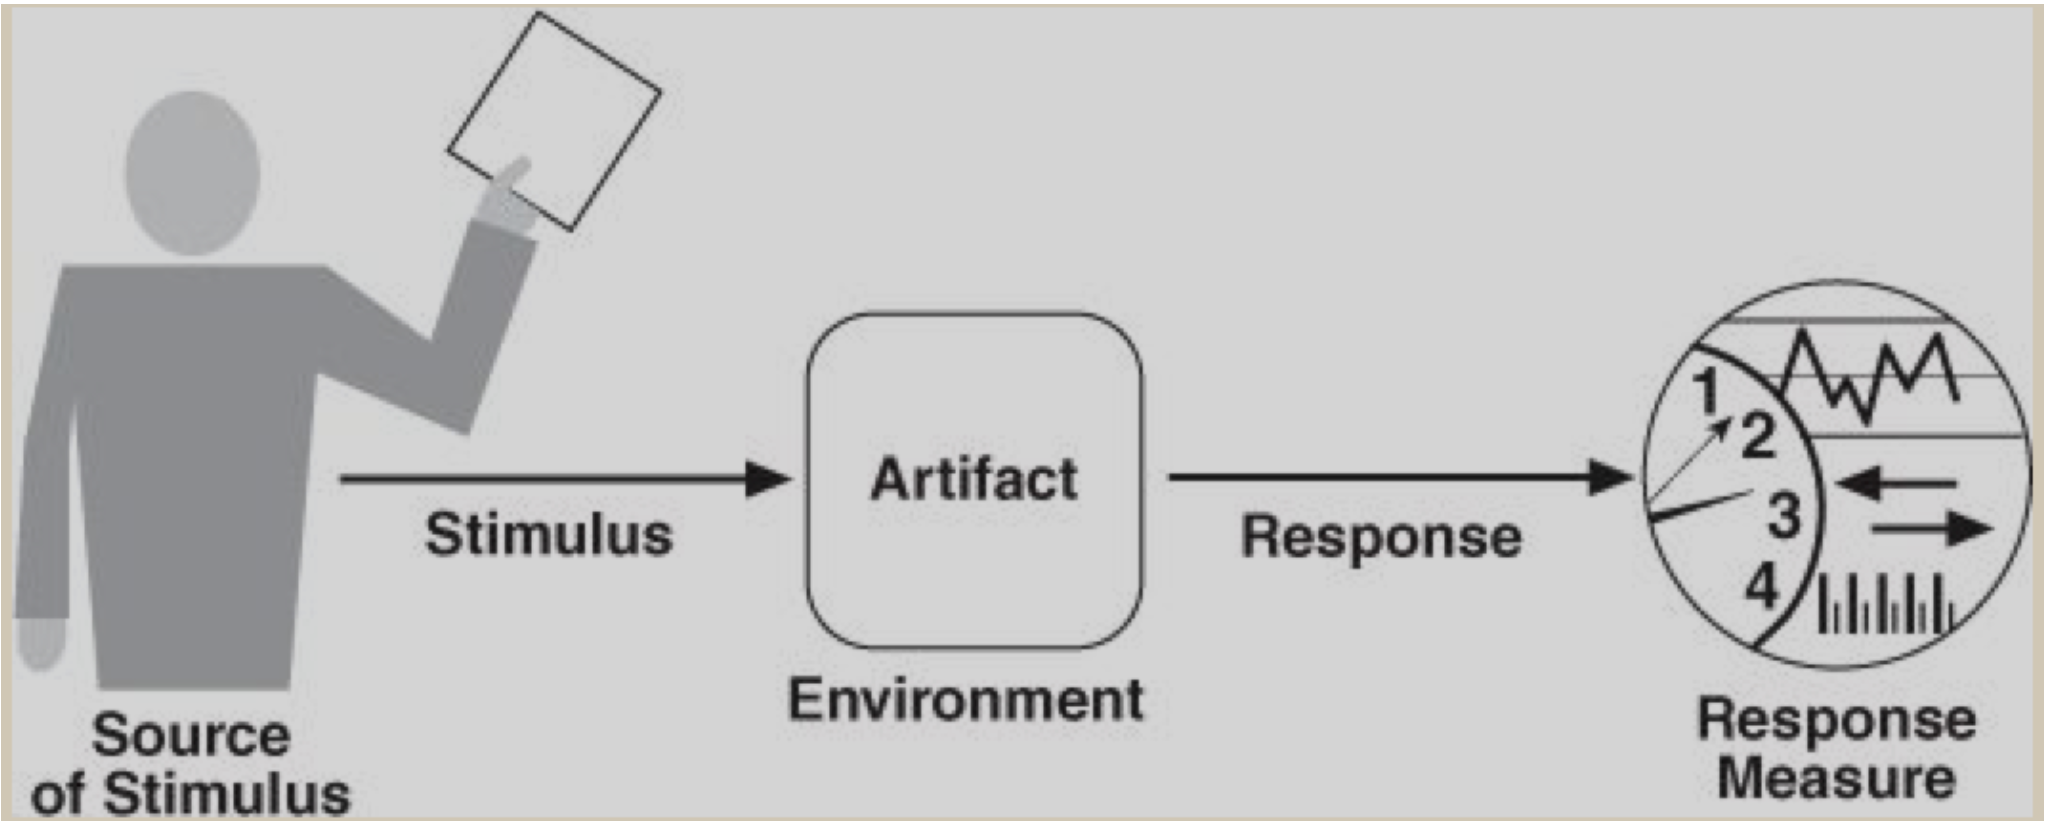
\includegraphics[scale=0.3]{aimages/genreralqascenario.png}
\caption{\label{tab:widgets}Security Architectural Tactics}
\end{figure}

\section{Architectural Design Decisions}
\subsection{Allocation of resposibilities}
For security-system responsibilities do the following:
\begin{itemize}
\item Ensure all actors have identities(like roles)
\item Authenticate identities to apprppriate actors.
\item Check and Ensure Authorization
\item Ensure Data Encryption
\item Log attempts, successes, failures and other senitive oprations.
\end{itemize}
\subsection{Coordination Model}
The following things in the coordination model need to be acoounted for:
\begin{itemize}
\item Ensure coordination mechanisms use authentication and 
\item Ensure the coordination model is not vulnerable to tampering, interception, impoersonation.
\item The model data involved is encrypted.
\item Monitor level of demand for communication to identify excessive demands
\end{itemize}
\subsection{Data Model}
\begin{itemize}
\item Ensure There is a vald data model that disallows invalid data flows.
\item Ensure Logging of access, modification and attempted access or modification.
\item Data is protected in flight at rest using appropriate encryption
\item Ensure appropriate backup/recovery mechanisms are in place. 
\end{itemize}

\subsection{Mapping among Architectural Elements}
\begin{itemize}
\item Explore and be wary be wary how different mappings change the way users can access resources.
\item Ensure for all the mappings, the responsibilities(authorization, logging,encryption etc) are preserved.
\item Ensure recovery from attack is possible.
\end{itemize}
\subsection{Resource Management}
\begin{itemize}
\item explore teh overheads resulting from responsibilities(logging, encryption, recovery etc).
\item Analyse how a user can make demands on a critical resource.
\item Make sure malicious use of resources is detected and managed.
\item Identify and manage the potential fot corruption/contamination.
\item explore the potential for resource use to be used as a covert channel to trnasmit data.
\item limite resources used to manage sttemps at unauthorised use !!surely depends on use case?!!.
\end{itemize}
\subsection{Binding Time}
\begin{itemize}
\item Explore the consequesces of varying binding times on the ability to trust actor or components.
\item place mechanisms to ensure trust given in bindin time.
\item Explore impact on resource use, capacity/throughput, response time.
\item Ensure the time bindings are ensured with all resposibilities(authorization, logging,encryption etc).
\item Explore the potential of variation in binding time as a covert channel.
\end{itemize}

\subsection{Choices of Technologies}
\begin{itemize}
\item  Ensure limitations of technologies are understood and the potential for future compromise is well identified.
\item Ensure your chosen technologies support the tactics you want to deploy to protect the system.
\end{itemize}
\end{document}